%----------------------------------------------------------------
%
%  File    :  appendix.tex
%
%  Authors :  Keith Andrews, IICM, TU Graz, Austria
%             Manuel Koschuch, FH Campus Wien, Austria
% 
%  Created :  22 Feb 96
% 
%  Changed :  30 Oct 2008
%  !TEX root = ./thesis.tex
%----------------------------------------------------------------
\renewcommand*{\lstlistlistingname}{Codeverzeichnis}
\chapter{Anhang/Ergänzende Information}
\label{chap:app}
	% \begin{figure}[h!]
	% 	\centering
	% 	\begin{subfigure}
	% 		\centering
	% 		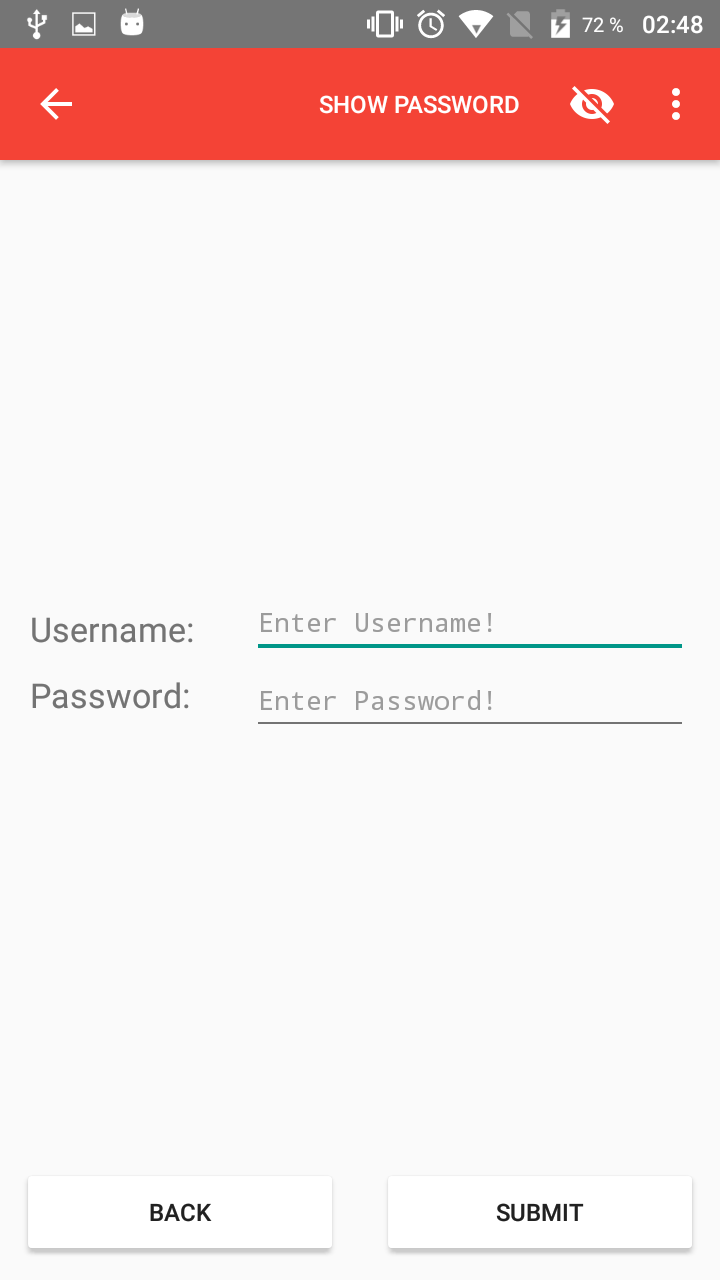
\includegraphics[width=.3\textwidth]{images/stm32kb-loginscreen.png}
	% 	\end{subfigure}
	% 	\label{fig:nope}
	% \end{figure}
	\begin{figure}[h!]
		\centering
		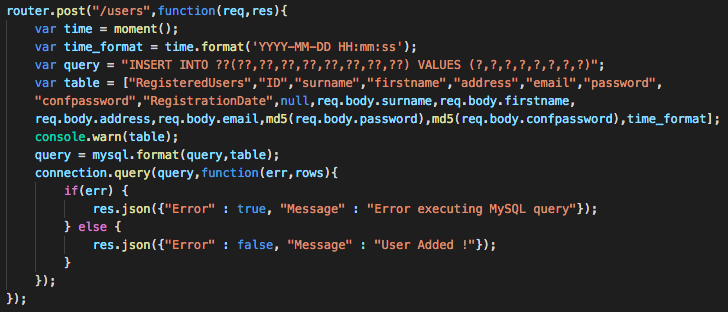
\includegraphics[width=1\textwidth]{images/restfull-server-code.png}
		\caption{RESTful - Server code - User Anlegen}
		\label{fig:serversidecode}
	\end{figure}

	\begin{lstlisting}[caption={Messung der Kommunikationszeit - MCKB PCL},label={lst:measurecom},captionpos=b,style=csharp]
protected override async void OnAppearing(){
    // Measing how long a request takes - START
    DateTime Jan1970 = new DateTime(1970, 1, 1, 0, 0, 0, DateTimeKind.Utc);
    TimeSpan javaSpan = DateTime.UtcNow - Jan1970;
    var time = DateTime.Now.Millisecond.ToString();
    var time3 = DateTime.UtcNow.ToString();
    System.Diagnostics.Debug.WriteLine(javaSpan + " Sending Request");
    var content = await _client.GetStringAsync(Url);
    var articles = JsonConvert.DeserializeObject<List<Article>>(content);
    DateTime Jan19702 = new DateTime(1970, 1, 1, 0, 0, 0, DateTimeKind.Utc);
    TimeSpan javaSpan2 = DateTime.UtcNow - Jan19702;
    var time2 = DateTime.Now.Millisecond.ToString();
    var time4 = DateTime.UtcNow.ToString();
    System.Diagnostics.Debug.WriteLine(javaSpan2 + " Received Request");
    // Measing how long a request takes - END
...}
	\end{lstlisting}

	\begin{lstlisting}[caption={MCKB Code-behind - Webservice Call},label={lst:mckbcodereg},captionpos=b,style=csharp]
...
namespace MCKB{
    public partial class MainPage : TabbedPage {
        private const string Url = "http://m4xwe11o.ddns.net:8000/api/articles";
        private HttpClient _client = new HttpClient();
        private ObservableCollection<Article> _articles;
		...
        protected override async void OnAppearing(){
        	...
            var content = await _client.GetStringAsync(Url);
            var articles = JsonConvert.DeserializeObject<List<Article>>(content);
			...
            _articles = new ObservableCollection<Article>(articles);
            ...
        }
    }
}

	\end{lstlisting}

	\begin{lstlisting}[caption={MCKB XAML Code für Registrierung},label={lst:mckbcodereg},captionpos=b,style=XML-Own]
<!--Tabbed Page two is for the registration of an user -->
<ContentPage Title="Register" Icon="icons8studentregistrationfilled.png">
    <ContentPage.Padding>
        <OnPlatform x:TypeArguments="Thickness" iOS="0,20,0,0" Android="0,0,0,0"></OnPlatform>
    </ContentPage.Padding>
    <StackLayout HorizontalOptions="FillAndExpand" VerticalOptions="Center" BackgroundColor="Silver" Padding="10,10,10,10">
        <Entry HorizontalTextAlignment="Center" Placeholder="Firstname"/>
        <Entry HorizontalTextAlignment="Center" Placeholder="Surname"/>
        <Entry HorizontalTextAlignment="Center" Placeholder="Address"/>
        <Entry HorizontalTextAlignment="Center" Placeholder="Email" Keyboard="Email"/>
        <Entry HorizontalTextAlignment="Center" Placeholder="Password" IsPassword="true"/>
        <Entry HorizontalTextAlignment="Center" Placeholder="Confirm Password" IsPassword="true"/>
        <StackLayout HorizontalOptions="Center" VerticalOptions="CenterAndExpand">
            <StackLayout Orientation="Horizontal" Padding="0,0,0,0">
                <Label Text="Accept AGB" VerticalOptions="Center"/>
                <Switch IsToggled="false" x:Name="accept" BackgroundColor="Gray" VerticalOptions="Center"/>
                <Button Text="REGISTER PAGE" IsEnabled="{Binding Source={x:Reference accept}, Path=IsToggled}" BackgroundColor="Gray"/>
            </StackLayout>
        </StackLayout>
    </StackLayout>
</ContentPage>
	\end{lstlisting}

	\begin{figure}[h!]
		\centering
		\begin{subfigure}
			\centering
			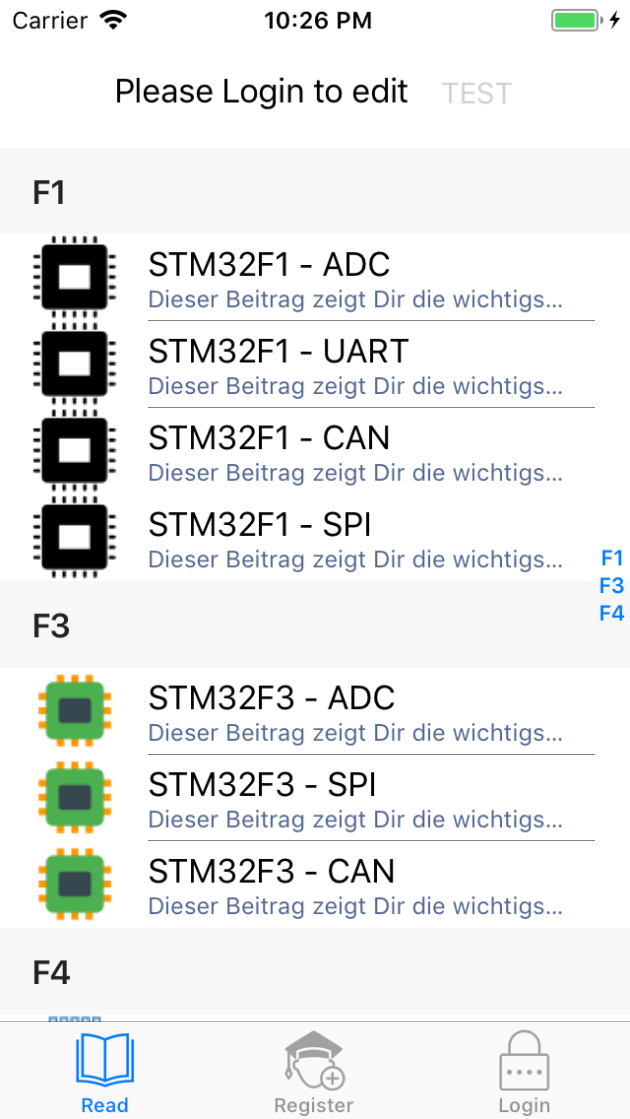
\includegraphics[width=.3\textwidth]{images/MCKB-iOS-Reading-Final.png}
		\end{subfigure}
		\begin{subfigure}
			\centering
			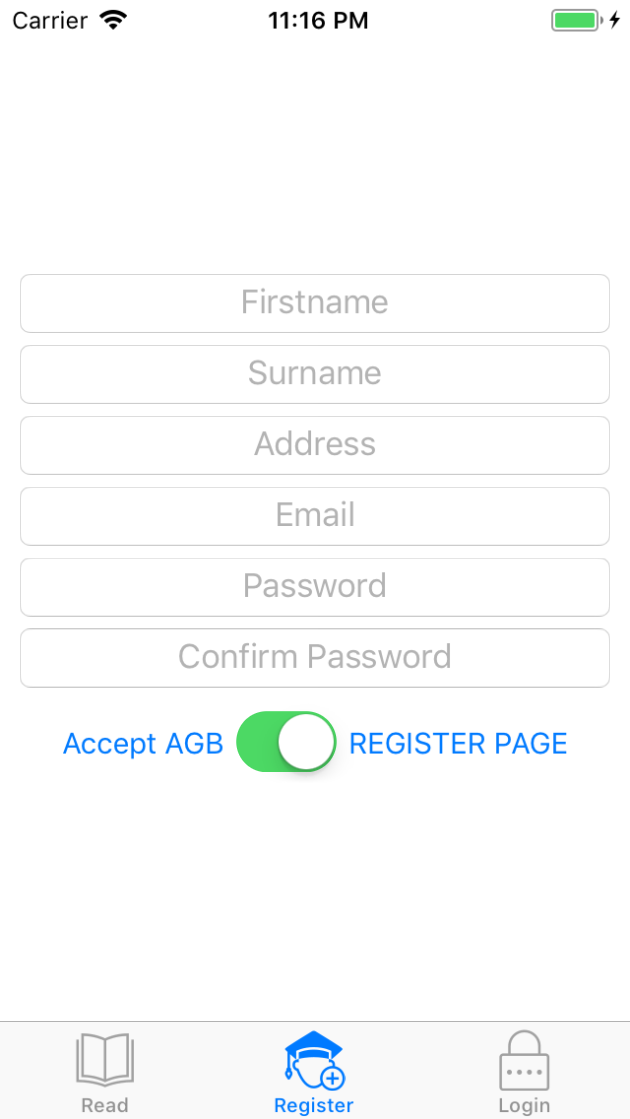
\includegraphics[width=.3\textwidth]{images/MCKB-iOS-Register-Final.png}
		\end{subfigure}
		\begin{subfigure}
			\centering
			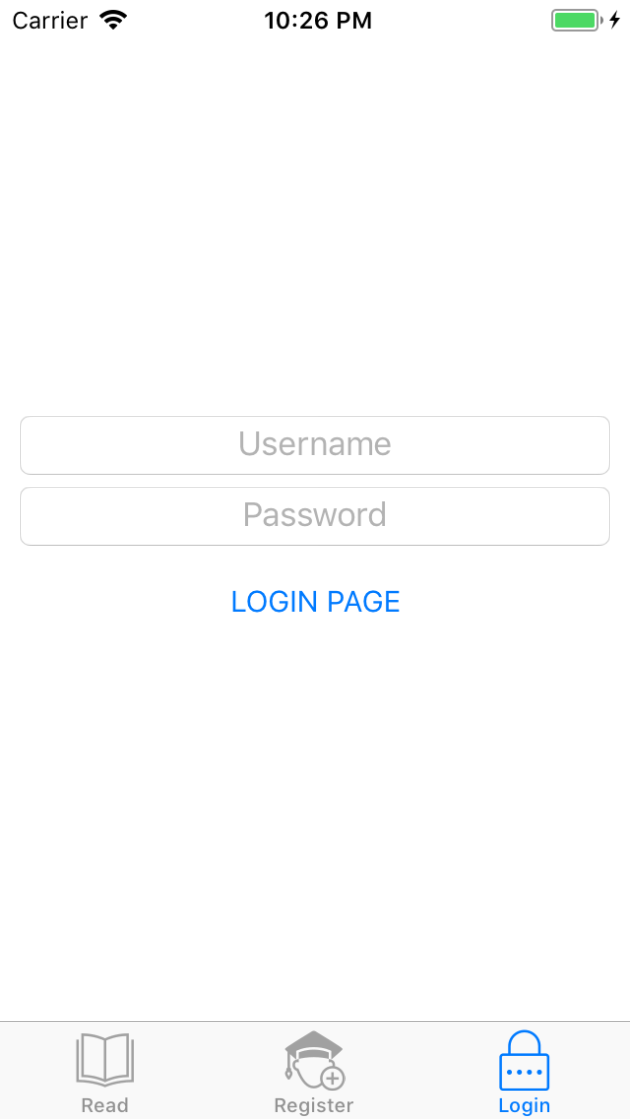
\includegraphics[width=.3\textwidth]{images/MCKB-iOS-Login-Final.png}
		\end{subfigure}
		\begin{subfigure}
			\centering
			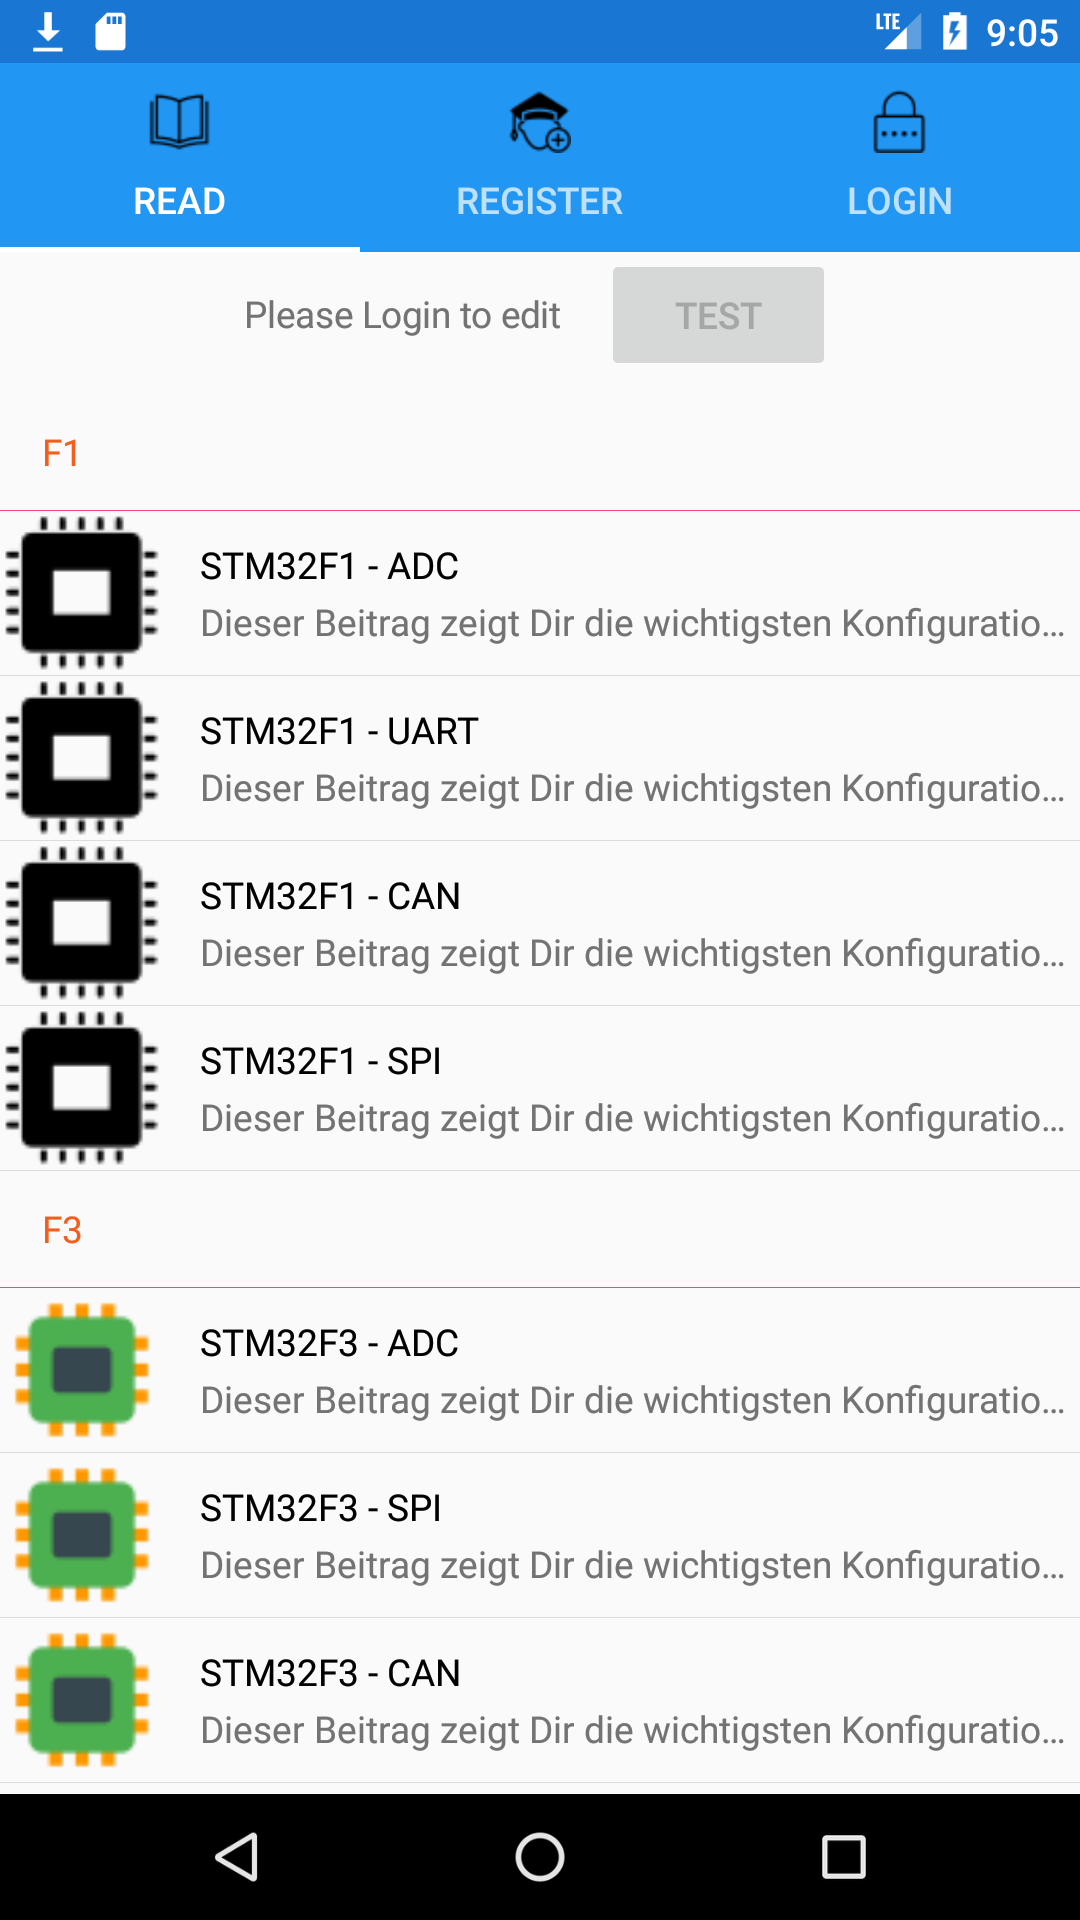
\includegraphics[width=.3\textwidth]{images/MCKB-Droid-Reading-Final.png}
		\end{subfigure}
		\begin{subfigure}
			\centering
			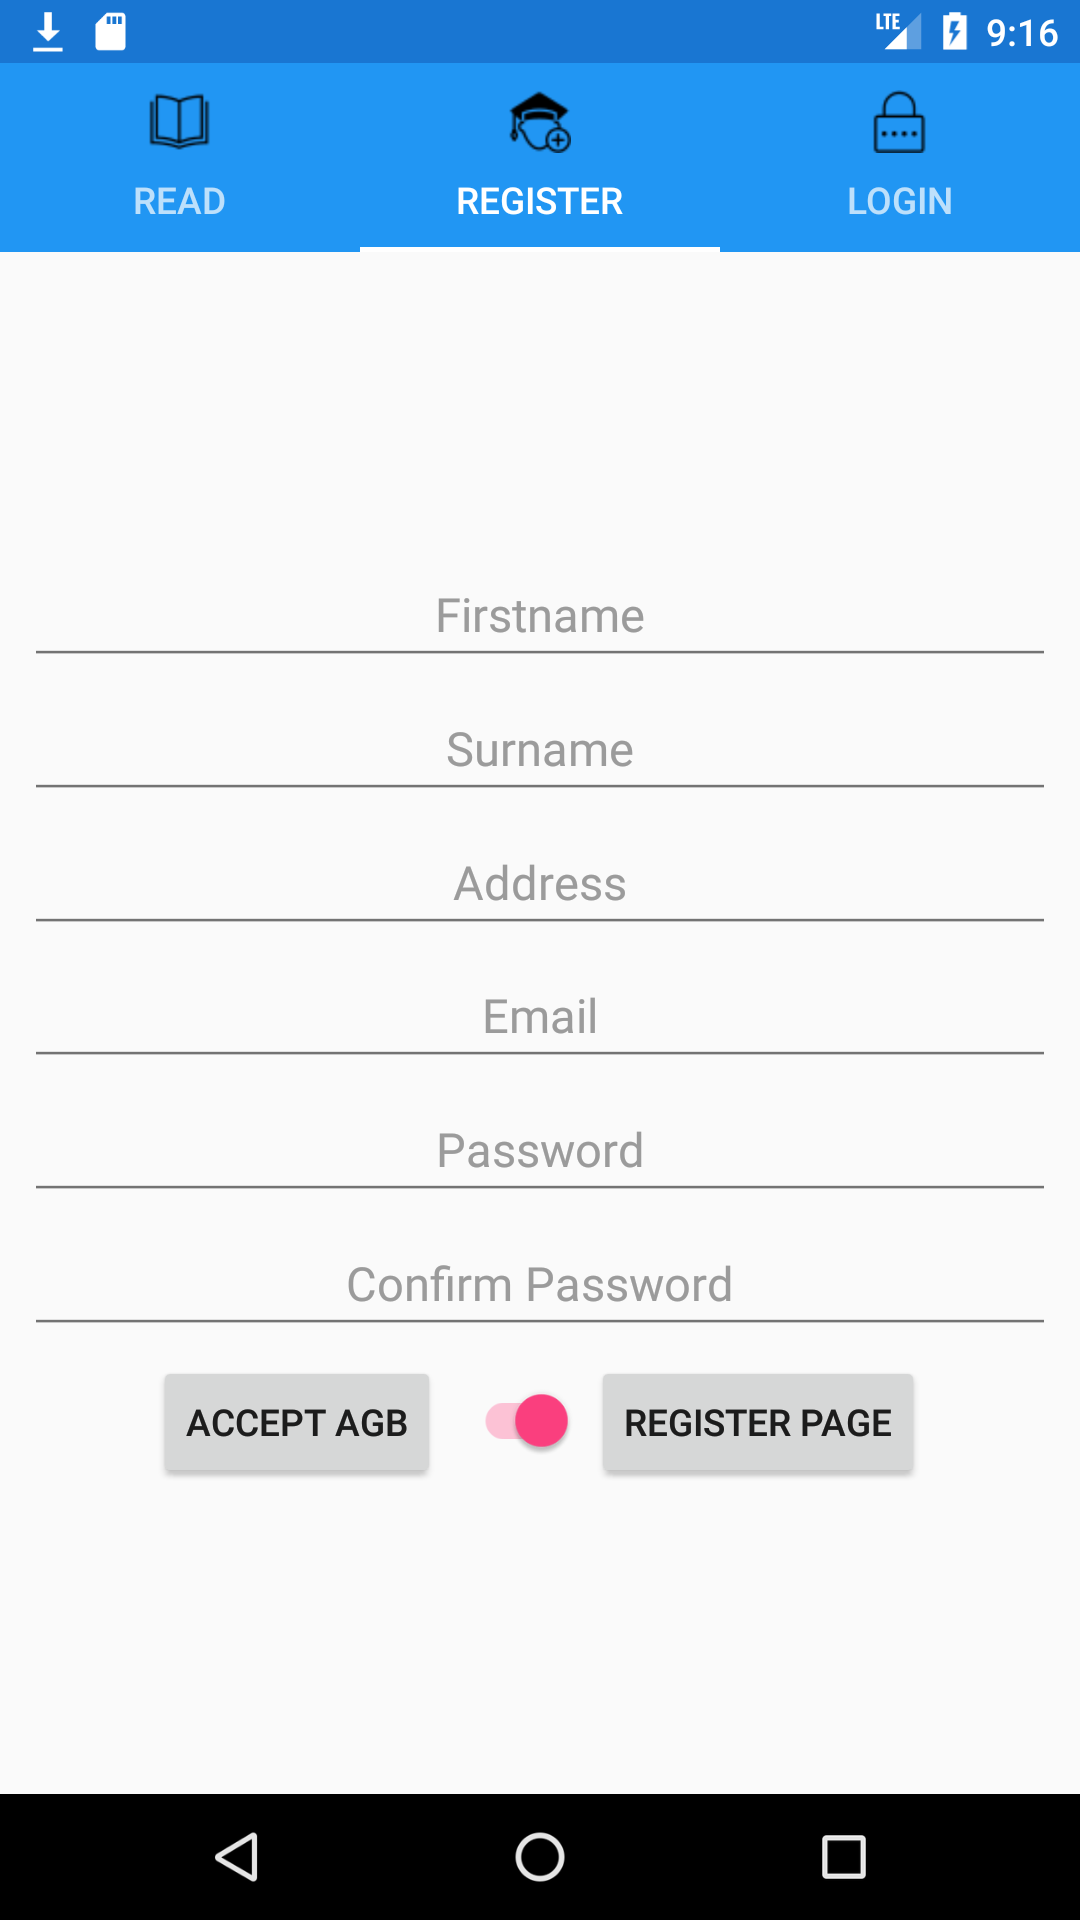
\includegraphics[width=.3\textwidth]{images/MCKB-Droid-Register-Final.png}
		\end{subfigure}
		\begin{subfigure}
			\centering
			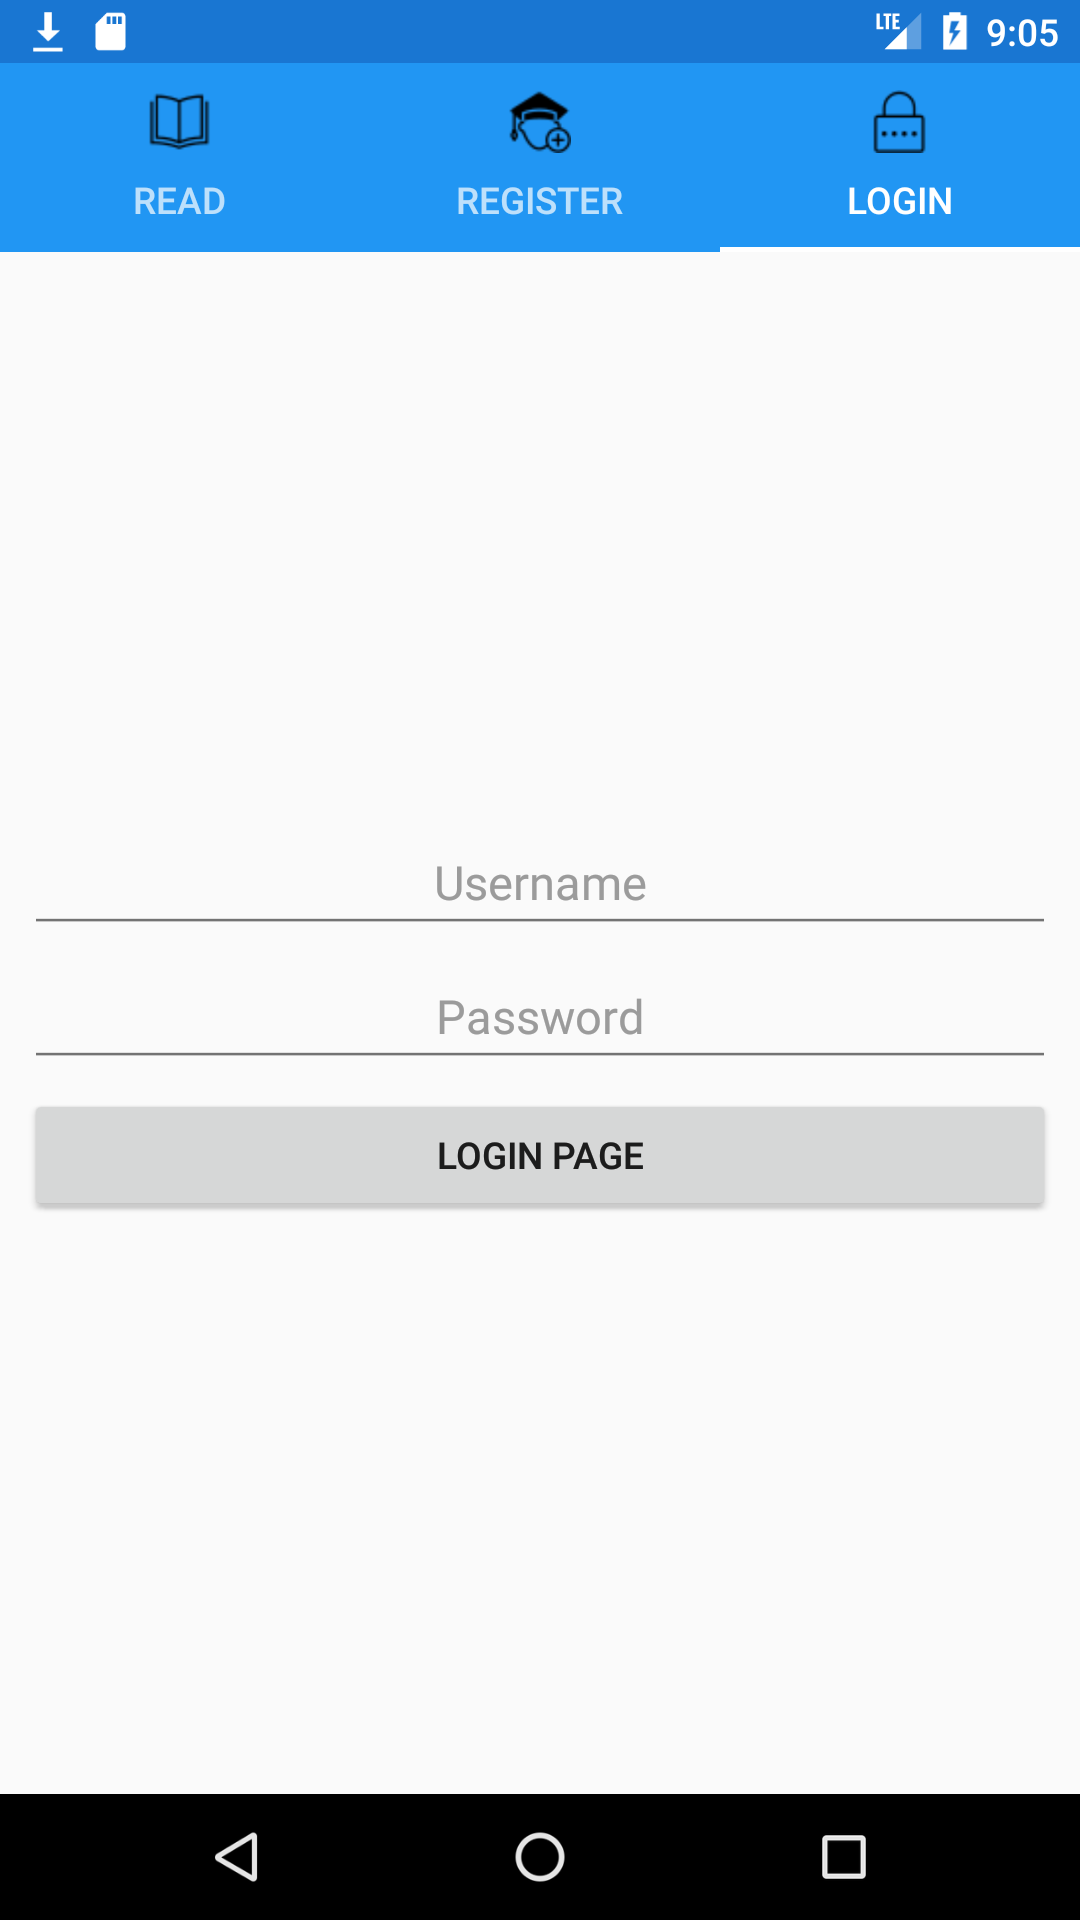
\includegraphics[width=.3\textwidth]{images/MCKB-Droid-Login-Final.png}
		\end{subfigure}
		\caption{Finales Design der MCKB App - Oben iOS / Unten Android}
		\label{fig:mckbAppfinal}
	\end{figure}
	
	\newpage
	\begin{lstlisting}[caption={MCKB - Design XAML Code},label={lst:mckbdesigncode},captionpos=b,style=XML-Own]
<?xml version="1.0" encoding="UTF-8"?>
<TabbedPage xmlns="http://xamarin.com/schemas/2014/forms" xmlns:x="http://schemas.microsoft.com/winfx/2009/xaml" x:Class="MCKB.MainPage">
    <!--Tabbed Page one is for the Artilces -->
    <ContentPage Title="Read" Icon="openbook.png">
        <ContentPage.Padding>
            <OnPlatform x:TypeArguments="Thickness" iOS="0,20,0,0" Android="0,0,0,0"></OnPlatform>
        </ContentPage.Padding>
        <StackLayout>
            <!--On top of the ListView to provide EDIT function -->
            <StackLayout>
                <StackLayout HorizontalOptions="Center" VerticalOptions="CenterAndExpand" Orientation="Horizontal">
                    <StackLayout.Padding>
                        <OnPlatform x:TypeArguments="Thickness" iOS="0,5,0,0" Android="0,0,0,0"></OnPlatform>
                    </StackLayout.Padding>
                    <Label Text="Please Login to edit" VerticalOptions="Center" HorizontalOptions="StartAndExpand"/>
                    <Button Text="Edit" IsEnabled="false" x:Name="editButton" Margin="10,0,0,0" Clicked="editButtonClicked"/>
                </StackLayout>
            </StackLayout>
            <ListView x:Name="articleListView" IsGroupingEnabled="true" GroupDisplayBinding="{Binding Title}">
                <ListView.ItemTemplate>
                    <DataTemplate>
                        <ImageCell Text="{Binding Title}" TextColor="Black" Detail="{Binding Description}" ImageSource="{Binding ImageUrl}"></ImageCell>
                    </DataTemplate>
                </ListView.ItemTemplate>
                <ListView.GroupHeaderTemplate>
                    <DataTemplate>
                        <TextCell Text="{Binding Title}" Detail="{Binding Description}" TextColor="#f35e20" DetailColor="#503026" />
                    </DataTemplate>
                </ListView.GroupHeaderTemplate>
            </ListView>
        </StackLayout>
    </ContentPage>

    <!--Tabbed Page two is for the registration of an user -->
    <ContentPage Title="Register" Icon="icons8studentregistrationfilled.png">
        <ContentPage.Padding>
            <OnPlatform x:TypeArguments="Thickness" iOS="0,20,0,0" Android="0,0,0,0"></OnPlatform>
        </ContentPage.Padding>
        <StackLayout HorizontalOptions="FillAndExpand" VerticalOptions="Center" Padding="10,10,10,10">
            <Entry HorizontalTextAlignment="Center" Placeholder="Firstname" x:Name="regfirstname"/>
            <Entry HorizontalTextAlignment="Center" Placeholder="Surname" x:Name="regsurname"/>
            <Entry HorizontalTextAlignment="Center" Placeholder="Address" x:Name="regaddress"/>
            <Entry HorizontalTextAlignment="Center" Placeholder="Email" x:Name="regemail" Keyboard="Email"/>
            <Entry HorizontalTextAlignment="Center" Placeholder="Password" x:Name="regpassword" IsPassword="true"/>
            <Entry HorizontalTextAlignment="Center" Placeholder="Confirm Password" x:Name="regconfpassword" IsPassword="true"/>
            <StackLayout HorizontalOptions="Center" VerticalOptions="CenterAndExpand">
                <StackLayout Orientation="Horizontal" Padding="0,0,0,0">
                    <Button Text="Accept AGB" VerticalOptions="Center" Clicked="showAgb"/>
                    <Switch IsToggled="false" x:Name="accept" VerticalOptions="Center"/>
                    <Button Text="REGISTER PAGE" IsEnabled="{Binding Source={x:Reference accept}, Path=IsToggled}" Clicked="sendRegistration"/>
                </StackLayout>
            </StackLayout>
        </StackLayout>
    </ContentPage>

    <!--Tabbed Page three is for the login -->
    <ContentPage Title="Login" Icon="icons8password.png">
        <ContentPage.Padding>
            <OnPlatform x:TypeArguments="Thickness" iOS="0,20,0,0" Android="0,0,0,0"></OnPlatform>
        </ContentPage.Padding>
        <StackLayout HorizontalOptions="FillAndExpand" VerticalOptions="Center" Padding="10,10,10,10">
            <Entry HorizontalTextAlignment="Center" Placeholder="Username" Keyboard="Text" x:Name="username"/>
            <Entry HorizontalTextAlignment="Center" Placeholder="Password" IsPassword="true" x:Name="password"/>
            <Button Text="LOGIN PAGE" Clicked="sendLogin"/>
        </StackLayout>
    </ContentPage>
</TabbedPage>
	\end{lstlisting}

% section zusätzliche_screenshots (end)



% (Hier können Schaltpläne, Programme usw. eingefügt werden.)
% Hier werden die Entwürfe zur Design der App gelistet sein.b
\clearpage

% --- List of Figures ----------------------------------------------------

\addcontentsline{toc}{section}{Abbildungsverzeichnis}
\listoffigures

\clearpage

% --- List of Tables -----------------------------------------------------

\addcontentsline{toc}{section}{Codeverzeichnis}
\lstlistoflistings

\addcontentsline{toc}{section}{Tabellenverzeichnis}
\listoftables

\clearpage

% --- Bibliography ------------------------------------------------------

\bibliographystyle{alpha}


% List references I definitely want in the bibliography,
% regardless of whether or not I cite them in the thesis.

\nocite{book:Xamarin.Forms-Succinctly}
\nocite{book:Xamarin.Forms-Essentials:}
\nocite{book:Cross-platform-UI-Development-with-Xamarin.Forms}
\nocite{book:Xamarin-Mobile-Application-Development}
\nocite{Amer2016}
\nocite{Oleksandr2015}
\nocite{8016193}
\nocite{Mukesh2016}
\nocite{Soylemez2017}
\nocite{Maximilian2017}

\addcontentsline{toc}{section}{Literaturverzeichnis}
\bibliography{thesis}

